\chapter{INTRODUCTION}

{\baselineskip=2\baselineskip


\section{Background of the Study}

Electricity is essential to everyday living, powering different activities and circumstances, especially in households, from lights and appliances to connectivity.  Electricity powers nearly every aspect of home living, being the most used energy source and notable expense among Filipino households, with a 94.8\% usage rate based on the Philippines Statistics Authority (2023). During frequent power interruptions, Filipino households face severe impacts from frequent power interruptions including comfort issues and disruption of work and livelihoods.  Many households rely on diesel generators as a temporary measure, but these are costly to run and contribute to noise and air pollution, indicating the need for other alternative measures for power sources.

According to Villamil et. al (2020), “The internet of things is an emerging technology that is currently present in most processes and devices, allowing to improve the quality of life of people.” As IoT continues to revolutionize daily living, solar energy, powered by innovations such as photovoltaic (PV) panels, plays a crucial role in shaping the future of global energy. Photovoltaic solar energy is rapidly becoming a key player in the global energy transition. This surge in demand and innovation paves the way for a more sustainable future, making solar energy a central focus in the race for renewable solutions. As highlighted by Sampaio and González (2017), "The capture of solar energy through photovoltaic (PV) panels to generate electricity has emerged as one of the most promising markets in renewable energy.”  In response to this, many systems utilize off-grid renewable energy; systems such as solar power systems are designed to provide electricity. This aligns with the study of Ramly, Jamal, Abd Ghafar, and Babu (2019), who highlighted that the “Emergency Portable Solar Power Supply is a product that uses a renewable energy source (sunlight) as the main source of electricity.”

Today's solar power systems offer many benefits. The technologies mentioned above can contribute to addressing key issues in the Philippines. They aim to reduce the impact of frequent power interruptions and emergencies, while promoting scalable renewable energy innovations for affected communities. Additionally, it contributes to sustainable energy systems by addressing the unique reliability challenges of off-grid and disaster-prone areas in the region.

 According to an article by Albay (2025), In the Philippines, the average Filipino household experiences 28 electricity supply interruptions in a year, due to frequent outages caused by plant breakdowns based on a report. The sudden or frequent power interruptions force households and businesses alike to rely on costly diesel generators as a backup power source. In August  2025, the National Grid Corporation of the Philippines (NGCP) reported an unscheduled power interruption affecting Camiguin and Misamis Oriental, which are home to 92,808 and 956,900 households based on the Philippine Statistics Authority (2020). The outage left thousands of households and businesses without power, mostly relying on diesel generators and various power sources. Addressing this gap in reliable energy access is crucial to providing communities with an affordable, sustainable power alternative and reducing the impacts of sudden interruptions. 

 Recent efforts to adapt solar-powered power supply systems show potential but face limitations. For instance, Gozano et al. (2023) designed a solar-based portable power supply with a modular battery pack. However, the portable power supply was shown capable of only supplying a lower energy load, such as charging mobile phones, mobile lighting and small auxiliary loads such as a small AM/FM radio. There were also shortcomings, such as the short lifespan of AC power whenever the battery pack reaches a certain voltage drop. 
 
 Innovations in solar-powered power supply systems offer a promising solution to these challenges. Bhatti et al. (2024) developed a portable solar station with integrated battery management and load monitoring system, having a power output of 200 W, and a 2x2 array of 50 W solar panels to provide electricity for basic necessities, in times of power interruptions due to natural disasters. Similarly,  the study by Ramly et al (2019) designed a portable solar power supply for emergency situations, supplying electricity up to 100W at one time, and utilizing Arduino Uno with Bluetooth module and voltage sensor to get the voltage readings integrated into a mobile application.  The said system lasted for two days without the need for charging. Despite these innovations, current solar-powered power supply systems still face limitations, such as low energy capacity, short battery lifespan, and restricted support for higher power loads.
 
 To bridge these gaps, this study proposes a solar-powered rental station for detachable power sources with a 2x2 solar panel array for energy harvesting, a LiFePO4 battery for reliable storage, and an inverter for AC power conversion. The system integrates an ESP32 microcontroller, integrating IoT mechanisms to manage operations, with GPS for location tracking and GSM for communication. A coin-slot mechanism with a solenoid lock ensures secure access, while a mobile app provides real-time monitoring of battery charge levels and system status. The compact and user-friendly design offers a sustainable solution for communities affected by frequent power interruptions.


\section{Statement of the Problem}

Air pollution is among the Philippines' most critical environmental issues, primarily caused by the use of fossil fuels. The Philippines' reliance on fossil fuels for electricity generation, particularly coal, contributes to elevated levels of air pollution. In 2025, coal accounted for approximately 52.7\% of the country's electricity generation, while natural gas contributed 20.1\%. This dependence on fossil fuels leads to the emission of pollutants that adversely affect air quality and public health. (LowCarbonPower, 2025). 

Electricity is a necessity for modern life. In Camiguin (served by CAMELCO) and certain parts of Misamis Oriental (served by MORESCO 2), the local community frequently experiences unscheduled power interruptions, occurring multiple times a week. This issue is consistent with research indicating that power interruptions are common in developing countries (Ibañez, 2024; Taniguchi, 2019), such as the Philippines, particularly in rural areas (Ibañez, 2024; Ali, 2016). These interruptions not only hinder productivity but also affect daily comfort in many households, making them very inconvenient and a source of frustration.

Despite the availability of off-grid setups, power banks, and small gasoline generators, these options are often limited by cost, power capacity, or environmental sustainability.  Furthermore, the reliance on fossil-fueled alternatives poses safety risks and contributes to pollution. In response, the government encourages a shift away from fossil fuel energy sources (Koons, 2024) and promotes the use of renewables, as outlined in the policy framework provided for in Republic Act (RA) No. 9513 or the “Renewable Energy Act of 2008”. Hence, there is a growing need for technological systems, such as solar-powered systems, to align with sustainability mandates. Studies show that the transition to greater use of renewables has wide-ranging implications (Villanueva, 2021), underscoring the importance of integrating supportive technologies into local environmental strategies.

Solar-powered systems have been introduced either as portable power supplies or as charging stations, yet existing systems face multiple limitations. Many of these are only capable of supplying low-energy loads, such as charging mobile phones, providing mobile lighting, or powering small auxiliary devices like AM/FM radios (Gozana et al., 2023). Additionally, the average cost of an off-grid setup is high (Boodoo, 2024), making it unaffordable for many households. Research also shows that solar-powered systems are commonly installed within the premises of the college campus (Catalan et al., 2019), but have not been widely initiated for communal purposes (Catalan et al., 2023). Furthermore, a notable gap exists in security, as many systems lack sufficient measures to prevent delinquent users from tampering with or vandalizing the system. These gaps, along with the promotion of solar-powered coin-operated charging stations in remote and island barangays, are highlighted by Catalan et al. (2023), as these areas often face significant challenges in power accessibility.

Given these limitations, there is a clear need for an innovative solar-powered rental system that is both affordable and scalable, while providing reliable energy access for households and public areas affected by frequent and unscheduled power interruptions. This study aims to design and develop a solar-powered rental station with detachable power sources, offering a sustainable and user-friendly alternative to conventional backup solutions, while also addressing the need for improved security features.

\section{Objectives of the Study}

In view of the above stated problem, the following objectives are:
\subsection{General Objectives}
\begin{itemize}
	\item To design and develop a solar-powered rental station with detachable power sources that serves as a sustainable and user-friendly solution for supplying electricity, specifically intended for communities experiencing frequent power interruptions. 
\end{itemize}
\subsection{Specific Objectives}
\begin{itemize}
	\item To design the system architecture that integrates photovoltaic panels, energy storage, and a power inverter, ensuring sufficient capacity for powering small to medium-scale appliances.
	\item To develop a functional prototype of the rentable station with a detachable power source, with a secure coin-operated or app-based access mechanism for rental use.
	\item To integrate GPS and GSM modules to support real-time location tracking, communication, and monitoring of rented units.
	\item To evaluate the system’s performance in terms of efficiency, portability, security, and user satisfaction in a rental-based context.
	\item To provide sustainable energy access through affordable and shared power sources powered by solar energy.
\end{itemize}

\section{Significance of the Study}

This project benefits a diverse range of stakeholders including: 

\textit{Community Residents} - Community residents will benefit from continuous access to electricity through the solar-powered portable power source. This system ensures the community residents can use essential household appliances and stay connected during power interruptions, improving their daily lives and overall comfort.

\textit{Environment} - This study contributes to environmental sustainability by promoting the use of solar energy, a renewable resource, instead of relying on fossil-fueled generators. The system reduces carbon emissions and pollution, aligning with global sustainability goals.

\textit{Future Researchers} - Future researchers will find this study helpful because it gives important information on how to create solar-powered portable charging systems with features like GPS tracking, coin/app payment, and real-time monitoring. 

\textit{SDG 7: Affordable and Clean Energy} - This system provides support in giving people access to energy that is affordable, reliable, and environmentally friendly by offering a solar-powered rental station that provides communities, especially those often experiencing blackouts, with a clean and low-cost source of electricity.

\textit{Industry, Innovation, and Infrastructure} - This helps achieve the goal of improving systems, creating new technologies, and building stronger infrastructure by using modern technologies, as well as solar energy, which helps in creating innovative solutions that give communities a reliable energy option during power interruptions.


\section{Scope and Limitations}

This research focuses on designing a solar-powered rental station with detachable power sources to provide reliable and sustainable electricity for communities in Camiguin and selected areas in Misamis Oriental, which face frequent power interruptions. The system integrates photovoltaic panels, energy storage, and a power inverter to power small to medium-scale appliances. The design will include a coin-operated or app-based access mechanism for renting the power sources.

The study will incorporate GPS and GSM modules for real-time location tracking and communication, ensuring efficient monitoring of rented units. The system will be evaluated for efficiency, portability, security, and user satisfaction, focusing on its performance in a rental context.	 By offering a solar-powered alternative, this targeted solution addresses a critical gap in providing reliable energy access for communities affected by frequent power interruptions.

However, the proposed system also has several limitations. The detachable power source is not capable of operating high-demand power appliances such as air conditioners and large electrical equipment due to its limited power capacity. It cannot be used to charge electric vehicles, including electric cars like Tesla, as these require significantly higher power input. The deployment of the system is limited only to selected areas that frequently experience power interruptions and have sufficient exposure to sunlight, as it cannot operate efficiently in locations without proper solar access. Additionally, the coin-operated mechanism cannot accept paper money bills, and the system does not dispense physical change; instead, any remaining balance or excess payment will be credited to the user’s mobile application account. Furthermore, the system is unable to operate during extreme weather conditions, such as typhoons, to ensure user safety and protect the equipment from potential damage.

\section{Conceptual Framework}

\begin{figure}[H]
	\centering
	\caption{Process flow on how the system operates}
	\label{fig:conceptualfra}
	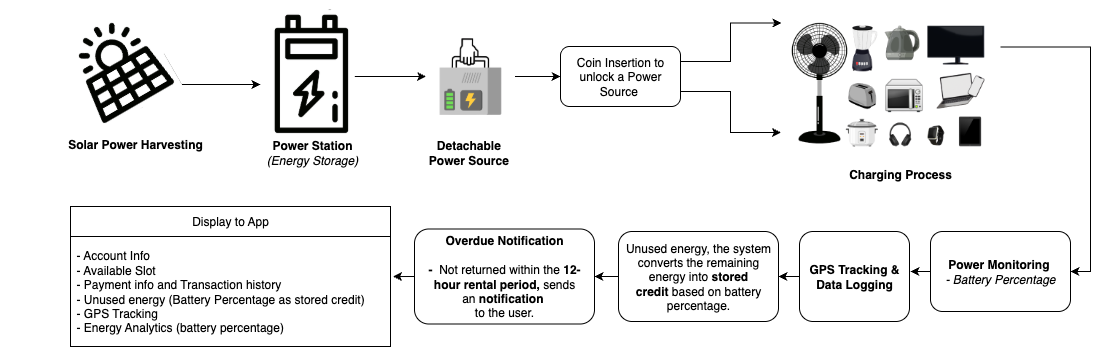
\includegraphics[width=1\textwidth]{figures/conceptual framework.png}
\end{figure}


Figure 1 illustrates the step-by-step process of how the proposed system functions, beginning with energy harvesting and ending with user access to the detachable power source. The process starts when photovoltaic (PV) panels capture solar energy and convert it into electricity. This electricity is then stored in the LiFePO4 battery, ensuring a reliable and long-lasting power supply. To make the stored energy usable for different devices, the system employs an inverter, which converts the direct current (DC) from the battery into alternating current (AC). Next, the ESP32 microcontroller, integrated with IoT mechanisms, monitors and manages the flow of energy. Through this control unit, real-time data such as battery charge level and system status can be tracked. Supporting modules such as GPS (for location tracking) and GSM (for wireless communication) enhance the monitoring and management of the system, particularly for rented power sources. For the rental mechanism, the system is equipped with a coin slot or app-based access system that unlocks the detachable power source through a solenoid lock. Once accessed, the user can rent and carry the power source for portable use, such as charging appliances or gadgets during power interruptions. The accompanying mobile application provides the renter with real-time updates on the battery level, usage duration, and system availability. Lastly, once the power source is returned, the system resets and recharges through solar harvesting, making it ready for the next user. This cyclical process ensures that the system remains sustainable, user-friendly, and reliable for communities experiencing frequent and unscheduled power interruptions.

\section{Definition of Terms}

\begin{description}

	\item[Internet of Things (IoT)] 
	A network of physical devices, such as sensors, appliances, and power sources, connected to the internet, enabling them to collect, send, and receive data for remote monitoring, control, and management.
	
	\item[Solar Energy] 
	Energy that is harnessed from sunlight using technologies such as photovoltaic (PV) panels, which convert sunlight into electricity, which is used to power the portable power sources.
	
	\item[Fossil Fuel] 
	Natural energy sources such as coal, oil, and natural gas, derived from the remains of ancient plants and animals, that are burned to produce energy but contribute to environmental pollution and climate change due to the emission of greenhouse gases.
	
	\item[Photovoltaic (PV) Panels] 
	Solar panels that convert sunlight into electricity, serving as the primary source of power generation for solar-powered systems.
	
	\item[Portable Power Station] 
	Compact, mobile units that provide electrical power for charging devices or operating appliances, often powered by renewable sources like solar energy and designed to be easily transported or moved.
	
	\item[Renewable Energy] 
	Energy derived from natural resources that are replenished on a human timescale, such as sunlight, wind, and geothermal heat, which are harnessed to produce electricity in an environmentally sustainable manner.
	
	\item[Off-grid power system] 
	A power system that operates independently from the main electricity grid, using renewable energy sources like solar or wind to provide electricity in areas without access to centralized power.
	
	\item[Solar harvesting] 
	The process of capturing sunlight using solar panels or other solar technologies and converting it into usable electrical energy, typically for storage in batteries or direct use.
	
	\item[Power Interruption] 
	TA temporary loss or disruption of electrical power, often due to faults, maintenance, or other technical issues in the power grid, affecting the availability of electricity to households or businesses.



\end{description}

}
